\chapter{Todo-rename-DNN}
\label{chap:dnn}
\section{Introduction}
The major Problem in \textit{Machine Learning} is that in most of real world applications, many factors of variation influence every single piece of data. Most of real world applications require us to disentangle these factors of variation in data and discard the ones which we don't care about. But it can be very difficult to extract these high level abstract features from raw data obtained. \textit{Deep learning} aims solves this problem in representation learning by introducing representations that are expressed in terms of other, simpler representations.

According to \cite{deng2014deep}, \textit{``Deep learning (deep structured learning or hierarchical learning) is a set of algorithms in machine learning that attempt to model high-level abstractions in data by using model architectures composed of multiple non-linear transformations"}.

Some of most successful deep learning methods uses principles \textit{Artificial Neural Networks (ANN)}. Different deep learning architectures which uses principles \textit{ANNs} such as Convolutional Neural Networks (CNNs), and Deep Belief Networks (DBN) have been applied to different  fields like computer vision, automatic speech recognition and  natural language processing where produced state-of-the-art results.

In this chapter we fist introduces Deep Neural Network and its bacic concepts in \ref{sec:dnn:dnn}. Later we briefly discuss common DNN architecture like \textit{CNNs, DBN, etc}.

\section{Deep Neural Network}
\label{sec:dnn:dnn}
Artificial neural networks are family of statistical learning models inspired by the \textit{1959 biological model (by Nobel laureates David H. Hubel \& Torsten Wiesel)}. A \textit{Deep Neural Network (DNN)} is a form of  Artificial Neural Network with multiple hidden layers between the input and output layers. 


\subsection{Motivations for Deep Architectures}
The Major motivations for deep architectures are the following:

\subsubsection{Deep architecture of Brain}
One of major motivation of Deep Architectures is deep structure of brain. For example, study of visual cortex, shows areas which contains representation of the input, and signals flow from one area to the next. Each level represents the input at a different level of abstraction, with more abstract features further up in the hierarchy, defined in terms of the lower-level ones. Moreover, representation in brain is between dense distributed and local: they are sparse (only 1\% of neurons are simultaneously active). 

\subsubsection{Insufficient depth can hurt}
According to complexity theory of circuit, deep architectures is more efficient than shallow architectures in terms of computational elements and parameters required to represent some functions. \citep{bengio2007scaling}. \citet{haastad1987computational} found that a function (of $n$ inputs) which can be efficiently represented with $O(n)$ nodes with a depth $d$, requires an exponential number ($O(2^n)$) of nodes if depth is $d-1$. \citep{bengio2007greedy}

\subsubsection{Cognitive processes seem deep}
If you consider process of perceiving by humans, we always organize ideas and concepts hierarchically.  we first learn simple concepts and then compose them to represent more abstract ones. 


\subsection{General Deep Network Framework}
As discussed in Section \ref{sec:dnn:dnn} Deep Neural Network can be considered as Multilayer perceptron with many hidden layers. Standard learning strategy of MLP contains following steps:
\begin{itemize}
\item The weights of Neural network is initialized by random values
\item Apply gradient descent using back-propagation (BP) algorithm.
\end{itemize}
But Apart from few exceptions, researchers soon found out that an MLP of more
than two hidden layers often failed \cite{bengio2007greedy} due to a well-known fact that the MLP learning involves an extremely difficult non-convex optimization problem and a gradient-based local search used in the BP algorithm easily gets stuck in local minimum.

So a greedy layer-wise training algorithm was proposed by \citet{hinton2006reducing} to train Deep Networks. It contain following major steps:
\begin{itemize}
\item Pre-training one layer at a time in a greedy way. This unsupervised learning at each layer in a way that preserves information from the input and disentangles factors of
variation in data. This act as initialization step. Hence, instead of doing a random initialization, we perform careful initialization and reduce chance of getting stuck on local minima.
\item Then network is fine-tuned with respect to the ultimate criterion of interest which may be classification or regression task.
\end{itemize}

\section{Deep Belief Networks}
Hinton showed that Restricted Boltzmann Machines (RBMs) can be stacked and trained in a greedy manner to form so-called Deep Belief Networks (DBN) \cite{hinton2006reducing}. Deep Belief Network is graphical model which learns to extract a deep hierarchical representation of data. First, an unsupervised training is performed on each layer (RBM) in a greedy manner. Then fine-tune network based on a supervised training criterion.
\begin{figure}
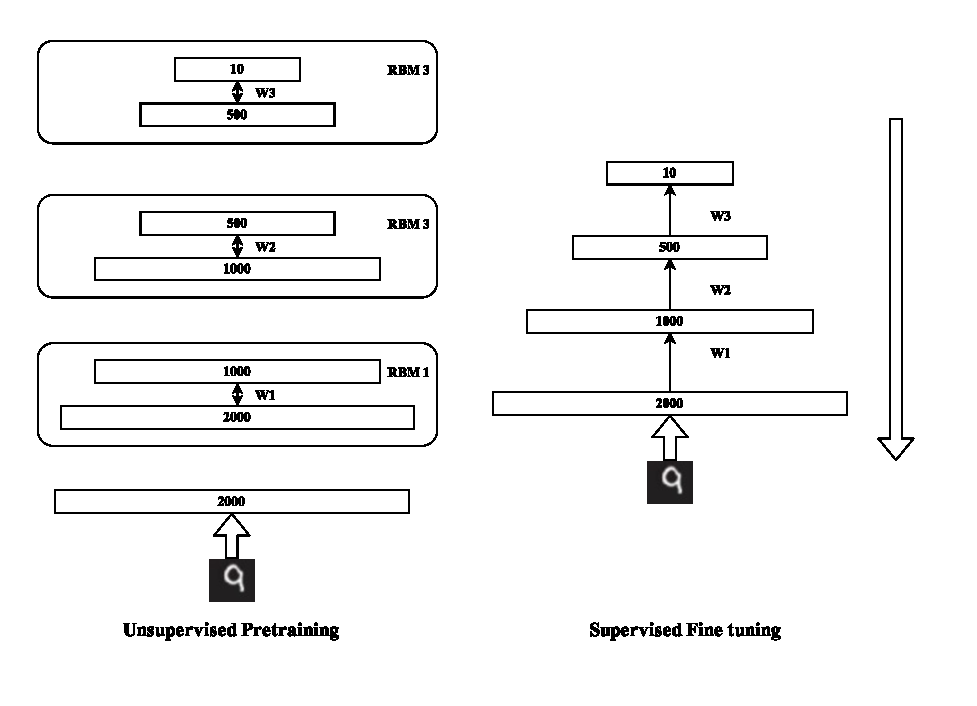
\includegraphics[scale=1]{./imgs/RBM_Train.eps} 
\caption{Training of DBN}
\end{figure}

RBM is an energy-based model. Energy based models has a scalar value (energy) to each configuration of variables. The Energy function $E(v,h)$ is defined as 